\section{Results}

\subsection{Multi-wavelength single-molecule co-localization (CoSMoS) methods}

We aim to improve methods for elucidating the molecular mechanisms of biochemical processes in vitro using multi-wavelength single-molecule fluorescence colocalization microscopy. For brevity, we call this experimental method CoSMoS (“colocalization single-molecule spectroscopy”). The key features of a CoSMoS experiment include: 1) One species of fluorescently labeled molecule (called the “target”) is tethered to the surface. Targets are immobilized at a surface density sufficiently low that the mean nearest-neighbor distance is large relative to the point-spread function (i.e., the diffraction-limited spot size) of the microscope. 2) Molecules, each species labeled with a different dye color, are added to the solution over the surface, typically at concentrations < 1 $\mu$M. When these “binder” molecules are freely diffusing in solution, they are invisible in TIRF. In contrast, when they are bound to the target, single binder molecules are detected as discrete fluorescent spots (Figure 1). The combination of features 1 and 2 means that formation of an individual binder-target complex is detected as spot appearance; dissociation of a binder-target complex is detected as spot disappearance \citep{friedman_viewing_2006, friedman_cosmos_analysis_2015}.

A representative CoSMoS experiment is illustrated by the example in Figure 1. In this experiment, we labeled the NusG protein with an orange dye. We then tethered to a microscope slide blue-dye-labeled DNA molecules at very low surface density (so that each molecule is resolved as a separate fluorescent spot) and observed real-time binding and dissociation of the other labeled molecules during the transcription process and its regulation.

\begin{figure}
\includegraphics[width=\linewidth]{fig}
\caption{A text-width example.}
\label{fig:view}
%% If the optional argument in the square brackets is "none", then the caption *will not appear in the main figure at all* and only the full caption will appear under the supplementary figure at the end of the manuscript.
\figsupp[Shorter caption for main text.]{This is a supplementary figure's full caption, which will be used at the end of the manuscript.}{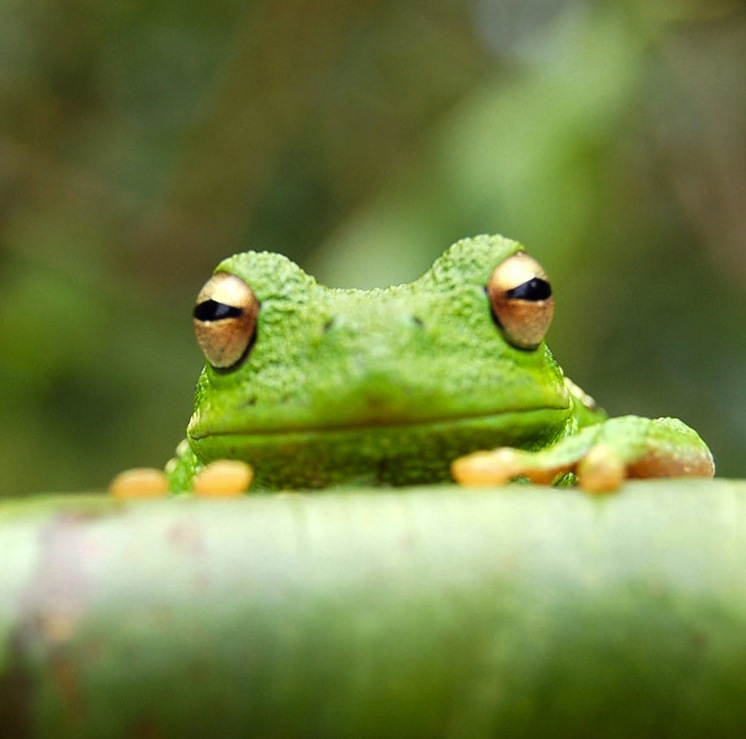
\includegraphics[width=6cm]{frog}}\label{figsupp:sf1}
\figsupp{This is another supplementary figure.}{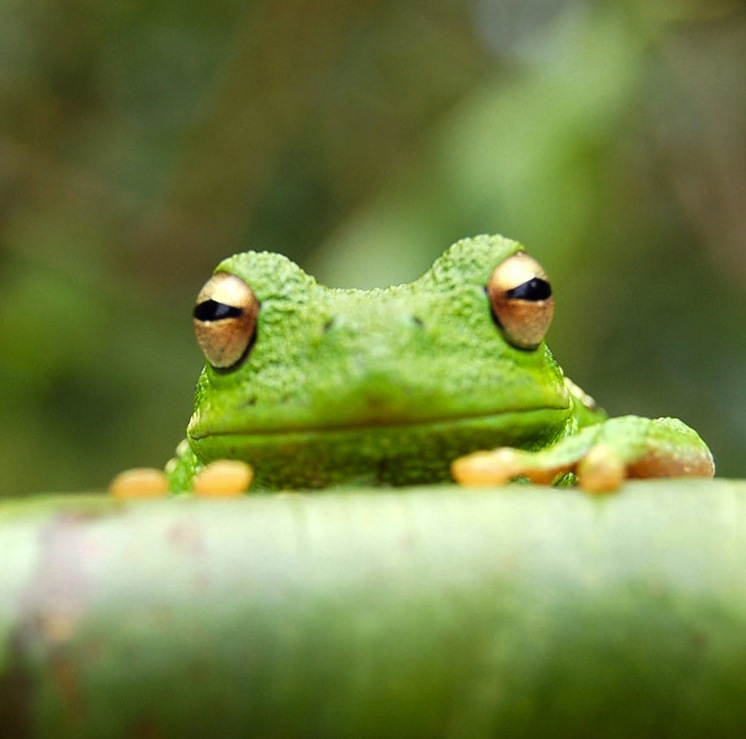
\includegraphics[width=6cm]{frog}}
\videosupp{This is a description of a video supplement.}\label{videosupp:sv1}
\figdata{This is a description of a data source.}\label{figdata:first}
\figdata{This is another description of a data source.}\label{figdata:second}
\end{figure}

\subsection{Comparison of Bayesisan method with heuristic spot thresholding}

We have done two types of performance comparison between the Bayesian method and the heuristic spot thresholding method. For the first performance comparison, a series of simulated data sets was constructed for a range of signal-to-noise values. For each S/N, a set of images with and without a 2-D Gaussian spots bound at the target and off-target were randomly generated. Intensity noise was generated using Gamma distribution to all simulated images.

Each data set was analyzed by both the Bayesian method and the heuristic spot thresholding algorithm (e.g., Figure 2, left). By comparison with the known “true” identities of the images, the accuracy of the resulting classifications was judged using a variety of specialized statistics for binary classification data, including true and false positive rates, true and false negative rates, and the Matthews Correlation Coefficient (MCC) \citep{fawcett_introduction_2006, matthews_comparison_1975}. The MCC statistic is widely regarded as a single overall, balanced measure which is meaningful even when the classes are of very different sizes. The MCC corresponds to the Pearson correlation coefficient between the estimated and “true” binary classifications. MCC=+1 represents a perfect prediction, MCC=0 a perfectly random prediction, and MCC=-1 indicates maximal disagreement between truth and estimation.

In a second comparison, images from real (i.e., not simulated) experimental data recordings were analyzed (Figure 3). Over a range of S/N, the Bayesian method gave image classification accuracy (as quantified by the MCC) similar to (or possibly better than) the heuristic spot thresholding algorithm The Bayesian method performs as well as the best existing CoSMoS data analysis method. Furthermore, Bayesian method achieves this performance automatically, with no adjustable parameters whatsoever, unlike the heuristic spot picker which attains this level of performance only after careful subjective trial-and-error manual adjustment of its three threshold parameters, a process that must be repeated tediously for each data set analyzed. Finally, our new Bayesian method produces a spot probability estimate for each image (not merely a Boolean spot/no spot determination) that can be used to inform subsequent kinetics calculations based on the results (e.g., the HMM analysis).

\subsection{Probabilistic modeling based on fundamental statistical analysis of data and priors}

To solve the problems with existing CoSMoS data analysis methods identified above, we have developed a new image-analysis-based approach that is accurate, objective, and built on a rigorous statistical approach to the CoSMoS image analysis problem. This TIBSD method is based on probabilistic modeling methodology. Bayesian model is a statistical model where probability is used to represent all uncertainty within the model, both for observed and hidden quantities in a system of interest. Bayes' theorem allows to perform inference on hidden variables given the observed data. The proposed first use of these methods for CoSMoS allows straightforward estimates of the uncertainty for estimated model parameters and rigorous quantitative testing of alternative image, noise, and kinetic models. “Time-independent” in the name TIBSD indicates that we ignore the time dimension of the recording -- the order of the images is arbitrary and does not affect the model, as each image is considered statistically independent of the others. We note that this time-independent method can naturally be extended into a time-dependent approach to both more accurately analyze the images and to directly obtain information about molecular kinetic mechanisms.  The proposed methods will eliminate the need for subjective image inspection and minimize the manual work required for CoSMoS data analysis.

\subsection{Time-independent Bayesian Spot Discrimination (TIBSD) method for analysis of CoSMoS data}

Unlike standard analysis methods for CoSMoS and single molecule FRET (smFRET), which are based on scalar intensity measurements derived from integration of emission in image regions of interest, our model fully uses information contained in the raw two-dimensional microscope images. The value of image data is proven in previous studies (Larry, Grunwald). To analyze the CoSMoS image classification problem within a Bayesian framework, one must define ideal image shapes for each class (image model) and choose a likelihood function for the observed data (noise model).

\subsubsection{Image classification}

The CoSMoS data set consists of a set of images where we have $N$ target sites ($n \in \{1,\dots,N\}$) each consisting of a series of $F$ different images in a recording ($f \in \{1,\dots,F\}$) (a “recording”). In each image, a binder molecule is either present on the single target molecule or absent. In addition, we explicitly model off-target binding of binder molecule. For simplicity  we assume that experimental conditions and image size were chosen so that at most only two spots ($K=2$) can exist in one image ($m_{nfk} \in \{ 0,1 \}$ -- existence indicator of the $k$-th spot). We treat the image classification problem as a data association problem by introducing an index variable for the on-target spot ($\theta_{nf} \in \{ 0,1,\dots,K \}$) where 0 means that on-target molecule is absent.

\subsubsection{Image model}

In the TIBSD method, we model the observed image data as a mixture of background image and “spot” images of binder molecules superimposed on background image. In particular, background image is modeled as a constant average background intensity $b_{nf}$; each spot image (2D point spread function) is modelled as an ideal (i.e., noiseless) 2-D Gaussian spot with integrated scalar intensity $h_{nfk}$ centered at ($x_{nfk}, y_{nfk}$). Each image is represented as a matrix (2D-array) $\mu^D_{nfij}$ of $P \times P$ pixels ($i,j \in \{1,\dots,P\}$). 

\textbf{\begin{equation*}
    \mu^{D}_{nfij} = b_{nf} + \sum_{k=1}^{K} \dfrac{m_{nfk}h_{nfk}}{2 \pi w^2_{nfk}} \exp{\left ( -\dfrac{(i-x_{nfk})^2 + (j-y_{nfk})^2}{2w^2_{nfk}} \right)}
\end{equation*}}

\subsubsection{Noise model}

 We use Gamma distribution as a noise model which is more flexible than Gaussian noise and can better approximate Poissonian camera noise. Scale parameter [add the variable name here?] of the Gamma distribution can be interpreted as a camera gain. Thus, the likelihood for the observed image can be expressed as:
 
 \begin{equation*}
     p(D_{nf}|\mu^D_{nfij},gain) = Gamma(D_{nf}|\mu^D_{nfij}/gain,1/gain)
 \end{equation*}

\subsubsection{Prior knowledge of colocalization accuracy}

Prior knowledge of colocalization accuracy can be directly incorporated into our model as priors for the center of the spot. On-target spots are localized around the target molecule within the experimentally determined accuracy and off-target spots are uniformly distributed within the image:

\begin{equation*}
    x_{nfk} \sim
\begin{cases}
    Beta^{\prime}(x_{nfk}|\mu^x=0,\nu^x_{prox}),& \text{if } \theta = k\\
    Beta^{\prime}(x_{nfk}|\mu^x=0,\nu^x_{flat}),& \text{otherwise}
\end{cases}
\end{equation*}

\begin{equation*}
    y_{nfk} \sim
\begin{cases}
    Beta^{\prime}(y_{nfk}|\mu^y=0,\nu^y_{prox}),& \text{if } \theta = k\\
    Beta^{\prime}(y_{nfk}|\mu^y=0,\nu^y_{flat}),& \text{otherwise}
\end{cases}
\end{equation*}


%\subsection{Image analysis, probabilities not binary classification}

%Expresses uncertainty. Allows downstream analysis. 

%\subsection{Flexible framework. Can select and use different models depending on the experiment}

%\subsubsection{Ability to jointly analyze different experimental conditions}

%\subsubsection{Models easily expandable to incorporate other data features}

\subsection{Software and hardware implementation}

The proposed research will provide more efficient ways to analyze large CoSMoS data sets. Technological developments such as faster, larger cameras \citep{huang_particle_nodate}, availability of fluorescent dyes with dramatically improved photostability (which increase the amount of data from a single experiment), and microscopes that efficiently collect single-molecule data at more wavelengths simultaneously \citep{friedman_viewing_2006} have all increased the sizes of CoSMoS datasets. Gelles lab studies of transient molecular binding events at high frame rates have produced >1 TB image data per experiment. Increasing data set sizes make it infeasible to use existing analytical methods. The code for the model and variational inference algorithm is written using Pyro probabilistic programming language. Pyro uses Pytorch as a backend for automatic differentiation and efficient computation of parallelizable vector-math operations on graphics processing units (GPUs). Our program is open-source and can be downloaded from the github repository.

\begin{comment}
\begin{table}[bt]
\caption{\label{tab:example}Automobile Land Speed Records (GR 5-10).}
% Use "S" column identifier to align on decimal point 
\begin{tabular}{S l l l r}
\toprule
{Speed (mph)} & Driver          & Car                        & Engine    & Date     \\
\midrule
407.447     & Craig Breedlove & Spirit of America          & GE J47    & 8/5/63   \\
413.199     & Tom Green       & Wingfoot Express           & WE J46    & 10/2/64  \\
434.22      & Art Arfons      & Green Monster              & GE J79    & 10/5/64  \\
468.719     & Craig Breedlove & Spirit of America          & GE J79    & 10/13/64 \\
526.277     & Craig Breedlove & Spirit of America          & GE J79    & 10/15/65 \\
536.712     & Art Arfons      & Green Monster              & GE J79    & 10/27/65 \\
555.127     & Craig Breedlove & Spirit of America, Sonic 1 & GE J79    & 11/2/65  \\
576.553     & Art Arfons      & Green Monster              & GE J79    & 11/7/65  \\
600.601     & Craig Breedlove & Spirit of America, Sonic 1 & GE J79    & 11/15/65 \\
622.407     & Gary Gabelich   & Blue Flame                 & Rocket    & 10/23/70 \\
633.468     & Richard Noble   & Thrust 2                   & RR RG 146 & 10/4/83  \\
763.035     & Andy Green      & Thrust SSC                 & RR Spey   & 10/15/97\\
\bottomrule
\end{tabular}

\medskip 
Source: \url{https://www.sedl.org/afterschool/toolkits/science/pdf/ast_sci_data_tables_sample.pdf}

\tabledata{This is a description of a data source.}

\end{table}
\end{comment}